\section{Methods} \label{sec: methods}

\subsection{Functional traffic network construction} \label{sec: network construction}
In order to analyze the percolation transition in dynamic traffic network, a framework is built based on percolation theory \cite{li2015percolation}. Instead of constructing a network based on the structure topology, only roads in the network with a speed greater than a specified threshold are considered functionally linked in this framework. The construction process is illustrated below:

Roads in real-world traffic networks can be divided into distinct states based on their speed. A road is considered as functional only if its velocity level meets a given demand. A variable threshold $ q \in [0, 1]$ is set to denote the speed demand of drivers at a given time. Measured data of speed is sorted during a long period of time for each road segment in increasing order, the 95 percentile is chosen as the standard maximal value of this road $v_{i j}^m$. Then the speed $v_{i j}(t)$ of each road from site $i$ to site $j$ at time is normalized to get the relative speed, $r_{i j} =v_{i j}(t)/v_{i j}^m$. Since the road network is a directed graph, $v_{i j}(t)$ is usually different from $v_{j i}(t)$ due to the direction of the traffic flow. For traffic state in each road segment, a comparison is made between the relative speed 
$r_{i j}(t)$ and the given threshold $q$. If $r_{i j}(t) \geq q$, the road section is functional because it satisfies demand; otherwise, it is dysfunctional and should be removed from the original road network.



\subsection{Critical threshold $q_c$}
We construct a functional network of the traffic dynamics from the original topology for any given $q$. If $q=0$, every road section meets demand, and the functioning traffic network is identical to the previous network. On the other hand, if $q=1$, since almost all the links are removed from the original network, the functional network becomes completely fragmented. The functional traffic network becomes diluted as $q$ grows from 0 to 1, which is known as "traffic percolation". $q_c(t)$ is the crucial threshold value of $q$ in traffic percolation, where the huge component of the dynamical network breaks down into fragmented local traffic clusters and the second biggest cluster reaches its maximum size \cite{li2015percolation, zeng2019switch}.


\begin{figure*}[hbt!]
\centering
\begin{subfigure}[t]{0.3\linewidth}
    \centering
    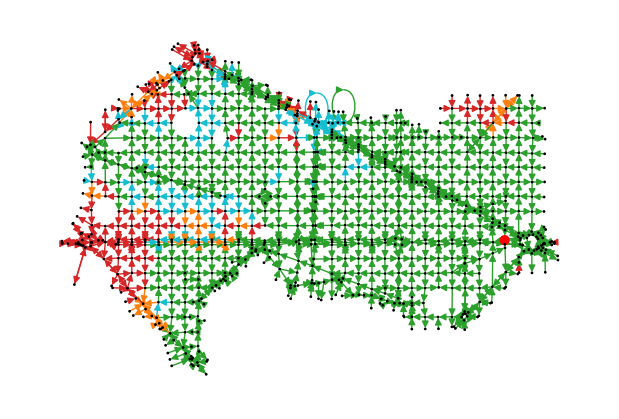
\includegraphics[width=\linewidth]{images/reachable/first_normal_1.png}
    \caption{Starting point 1, normal period}
    \label{fig: first normal reachable}
\end{subfigure}
\begin{subfigure}[t]{0.3\linewidth}
    \centering
    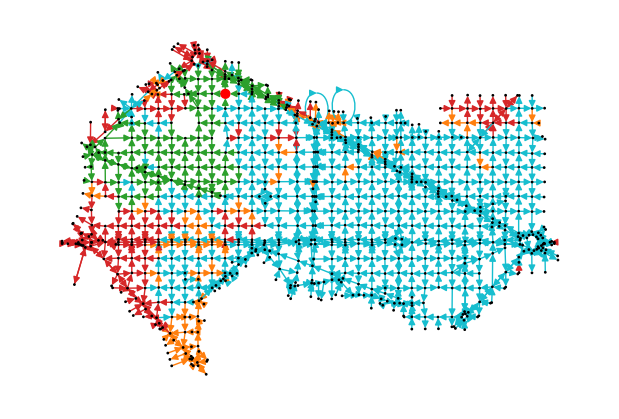
\includegraphics[width=\linewidth]{images/reachable/second_normal_1.png}
    \caption{Starting point 2, normal period}
    \label{fig: second normal reachable}
\end{subfigure}
\begin{subfigure}[t]{0.3\linewidth}
    \centering
    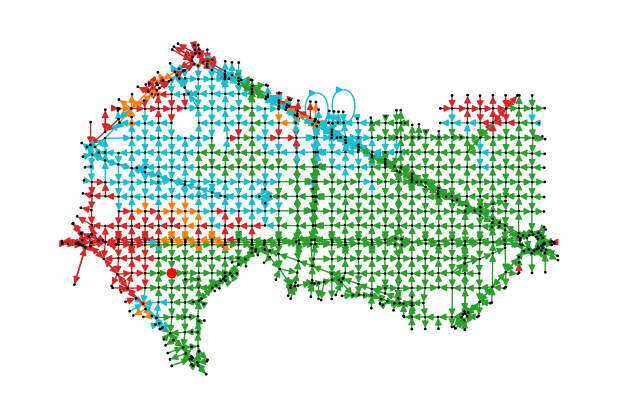
\includegraphics[width=\linewidth]{images/reachable/third_normal_1.png}
    \caption{Starting point 3, normal period}
    \label{fig: third normal reachalbe}
\end{subfigure}
\hfill
\begin{subfigure}[t]{0.3\linewidth}
    \centering
    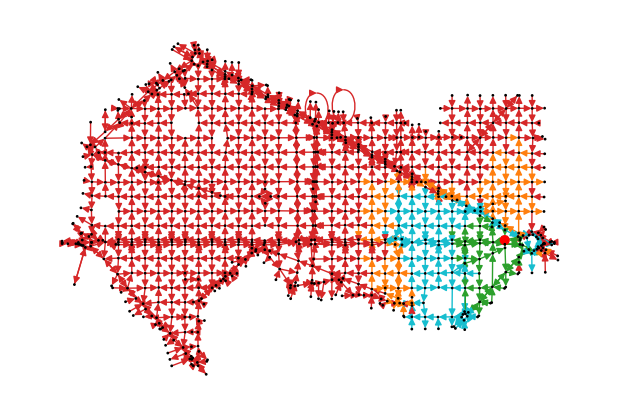
\includegraphics[width=\linewidth]{images/reachable/first_busy_1.png}
    \caption{Starting point 1, busy period}
    \label{fig: first busy reachable}
\end{subfigure}
\begin{subfigure}[t]{0.3\linewidth}
    \centering
    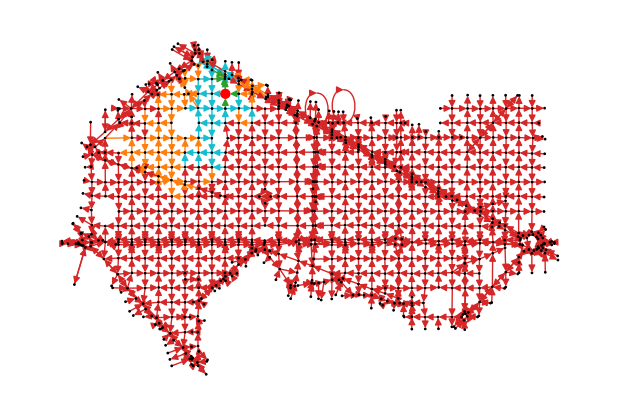
\includegraphics[width=\linewidth]{images/reachable/second_busy_1.png}
    \caption{Starting point 2, busy period}
    \label{fig: second busy reachable}
\end{subfigure}
\begin{subfigure}[t]{0.3\linewidth}
    \centering
    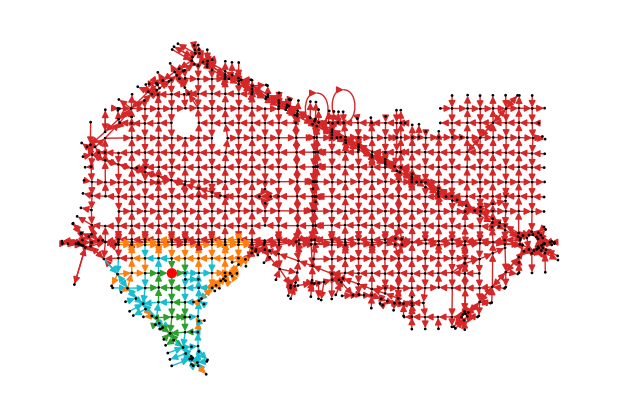
\includegraphics[width=\linewidth]{images/reachable/third_busy_1.png}
    \caption{Starting point 3, busy period}
    \label{fig: third busy reachable}
\end{subfigure}
\caption{The reachable area from different starting points (the red spot in green area). Green roads represent 1 minute reachable; blue for 2; orange for 3; and red for $>4$. We choose \textit{busy period} and \textit{normal period} mark.}
\hfill
\label{fig: reachable areas}
\end{figure*}




\subsection{Introduction of the bottleneck}
When we increase the $q$ value slightly above the crucial threshold $q_c$, several links are removed. While some links are removed accidentally, some links play an important function in linking distinct local traffic clusters in the traffic network. Only these links are considered as bottleneck roads, as their improvement will decide the critical threshold $q_c$ \cite{li2015percolation}.


\subsection{Network type and cluster power law}
City design varies in all cities. 2D grid is the most common topology, but it changes with different terrain and highway links. Specifically, the network would become more like a small-world model with more high speed links between distant locations. 

By the network constructed using the method stated in Section \ref{sec: network construction}, the connected components size and numbers follows a power rule as (\ref{eq: power law}) when we choose $q \simeq q_c$. 
\begin{equation} \label{eq: power law}
    n_s \sim s^{-\tau}
\end{equation}
where $n_s$ is the ratio between the number
of s-sized clusters and the total number of clusters; $s$ is the cluster size; and $\tau$ is the corresponding critical percolation exponent \cite{zeng2019switch}. 


The theoretical percolation exponent of a 2D grid is $\tau_{grid}^{(2)} = 2.05$, and for a small-world model is $\tau_{sw} = 2.5$ \cite{zeng2019switch, huang2018critical}. Thus, we can determine the type of network by comparing the empirical $\tau$. Since the traffic network is a spatial-temporal system \cite{zeng2019switch}, we check not only the static structure of the network, but also the evolution of $\tau$ across time. Generally, a road system is more resilient when it is able to maintain more high speed links under heavy traffic.
